\section*{\begin{center}{\Huge Appendix}\end{center}}
\addcontentsline{toc}{chapter}{Appendix}
$\\[0.5cm]$

\subsection*{Appendix A: Sample selection}
\addcontentsline{toc}{section}{A: Population selection}
\label{app:population_selection}
The following pages are generated from Jupyter notebook and document the sample selection procedure. The notebook is also available in the supplementary materials or at \url{https://github.com/sidgek/msoppgave}, together with the generated samples and files with the population of accepted papers they were generated from.
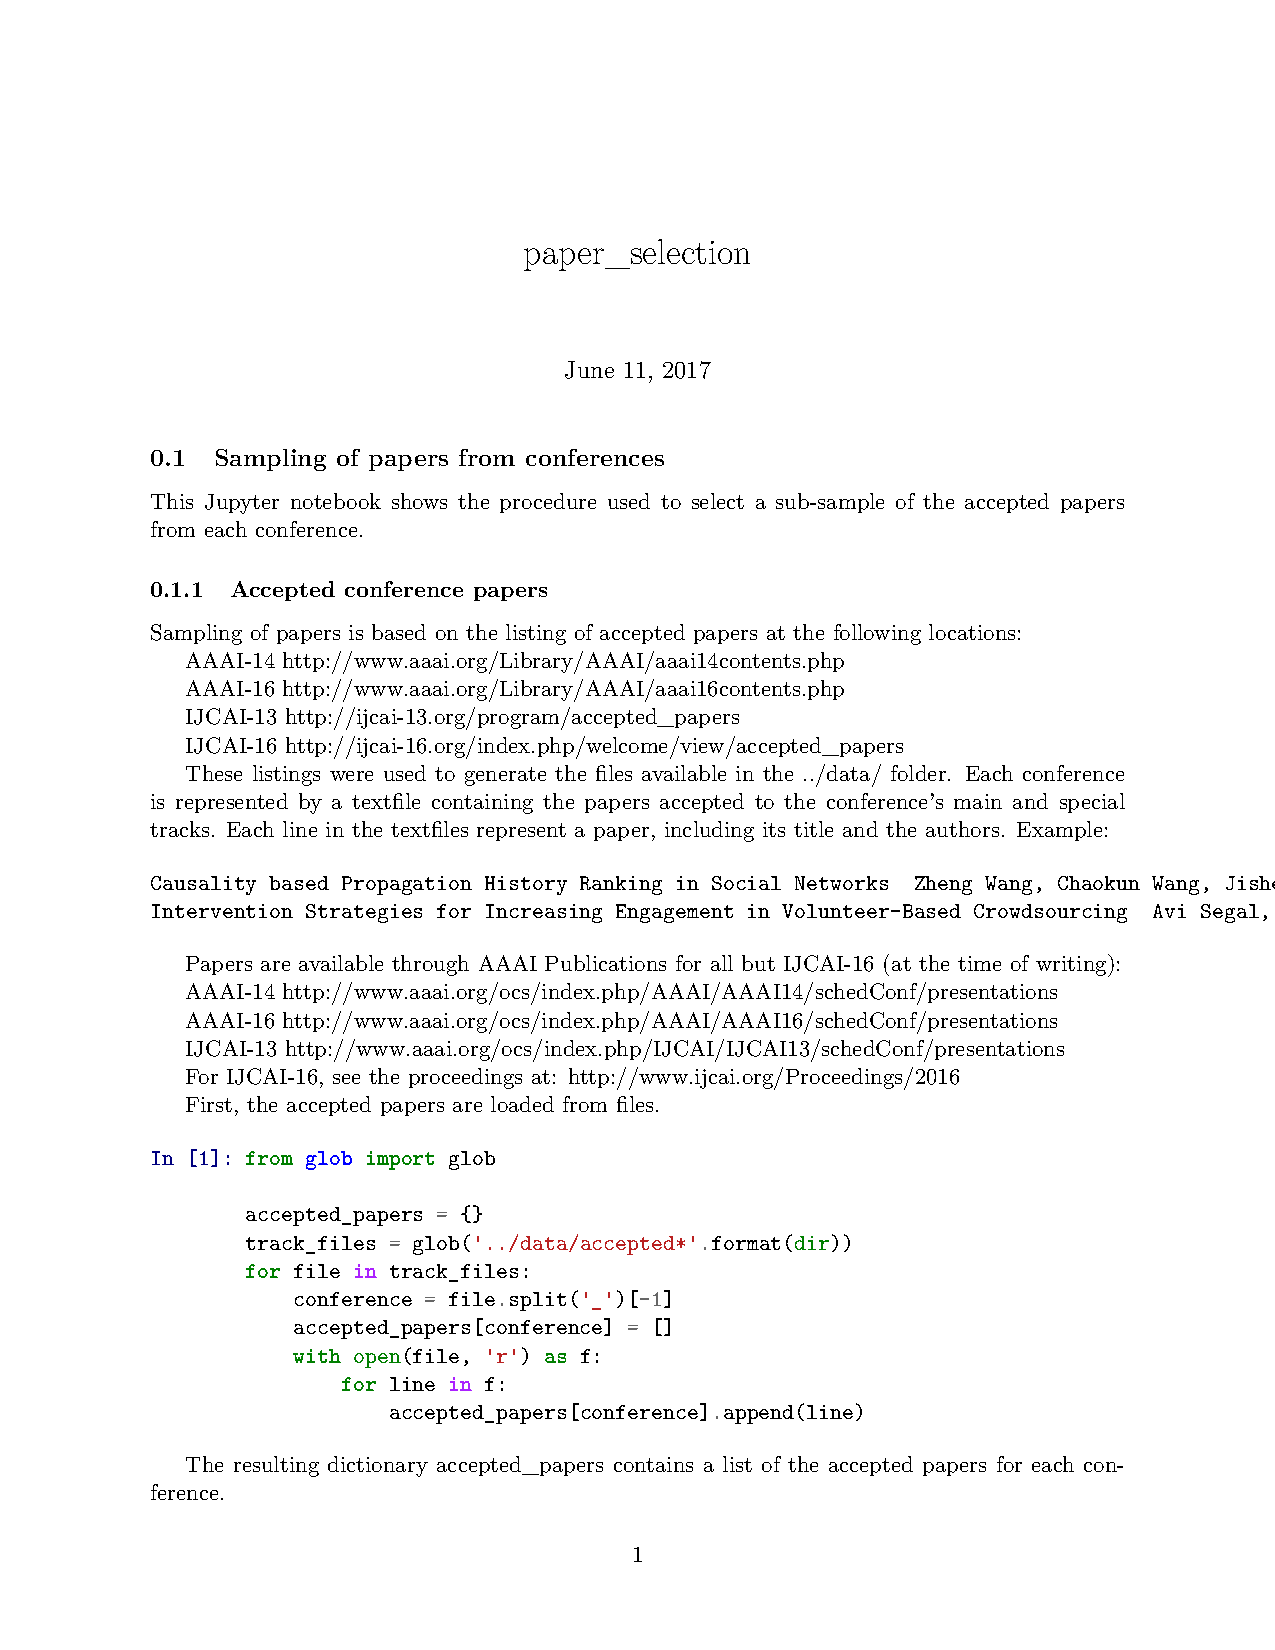
\includepdf[pages={-},scale=.8, pagecommand={}]{chapters/appendix_paper_selection.pdf}

\subsection*{Appendix B: Survey data}
\addcontentsline{toc}{section}{C: Analysis code}
\label{app:analysis_code}
Due to the amount of columns and rows in the dataset being impractical to add to the appendix, a sample of 10 abbreviated rows from the survey data is provided here to show the format. The entire evaluation dataset is provided as a .csv file in the supplementary materials and at \url{https://github.com/sidgek/msoppgave}.

\begin{table}[!h]
\begin{center}
    \begin{tabular}{ rlrrrrrrr }
    \textbf{index} & \textbf{title} & \textbf{resea..} & \textbf{result..} & \textbf{affil..} & .. & \textbf{evalu..} & \textbf{comme..} & \textbf{confe..} \\
    1 & A Gene.. & E & 1 & 0 & ..	& 1 & & IJCAI 16 \\
    2 & Provin.. & T &	1 &	0 & .. & 0 & & IJCAI 16 \\
    3 &	Effici.. &	E &	1 &	0 & .. & 1 & & IJCAI 16 \\
    4 &	Natura.. & E &	1 &	0 &	.. & 1 & & IJCAI 16 \\
    5 &	Learni.. & E &	1 &	0 & .. & 1 & & IJCAI 16 \\
    6 &	Dynami.. & E &	1 &	0 & .. & 1 & & IJCAI 16 \\
    7 &	A Unif.. & E &	1 &	0 &	.. & 1 & & IJCAI 16 \\
    8 &	Multi-.. & E &	1 &	0 & .. & 1 & & IJCAI 16 \\
    9 &	Change.. & E &	1 &	2 & .. & 1 & & IJCAI 16 \\
    10 & Model.. & E & 1 & 1 & .. & 1 & & IJCAI 16 \\
    \end{tabular}
\end{center}
\caption{Abbreviated sample of survey data.}
\label{tab:sample_survey_data}
\end{table}

\subsection*{Appendix C: Analysis code}
\addcontentsline{toc}{section}{C: Analysis code}
\label{app:analysis_code}
The following pages are generated from Jupyter notebook and document the procedure to generate the figures found in chapter~\ref{chap:results}. The notebook is also available in the supplementary materials or at \url{https://github.com/sidgek/msoppgave}.
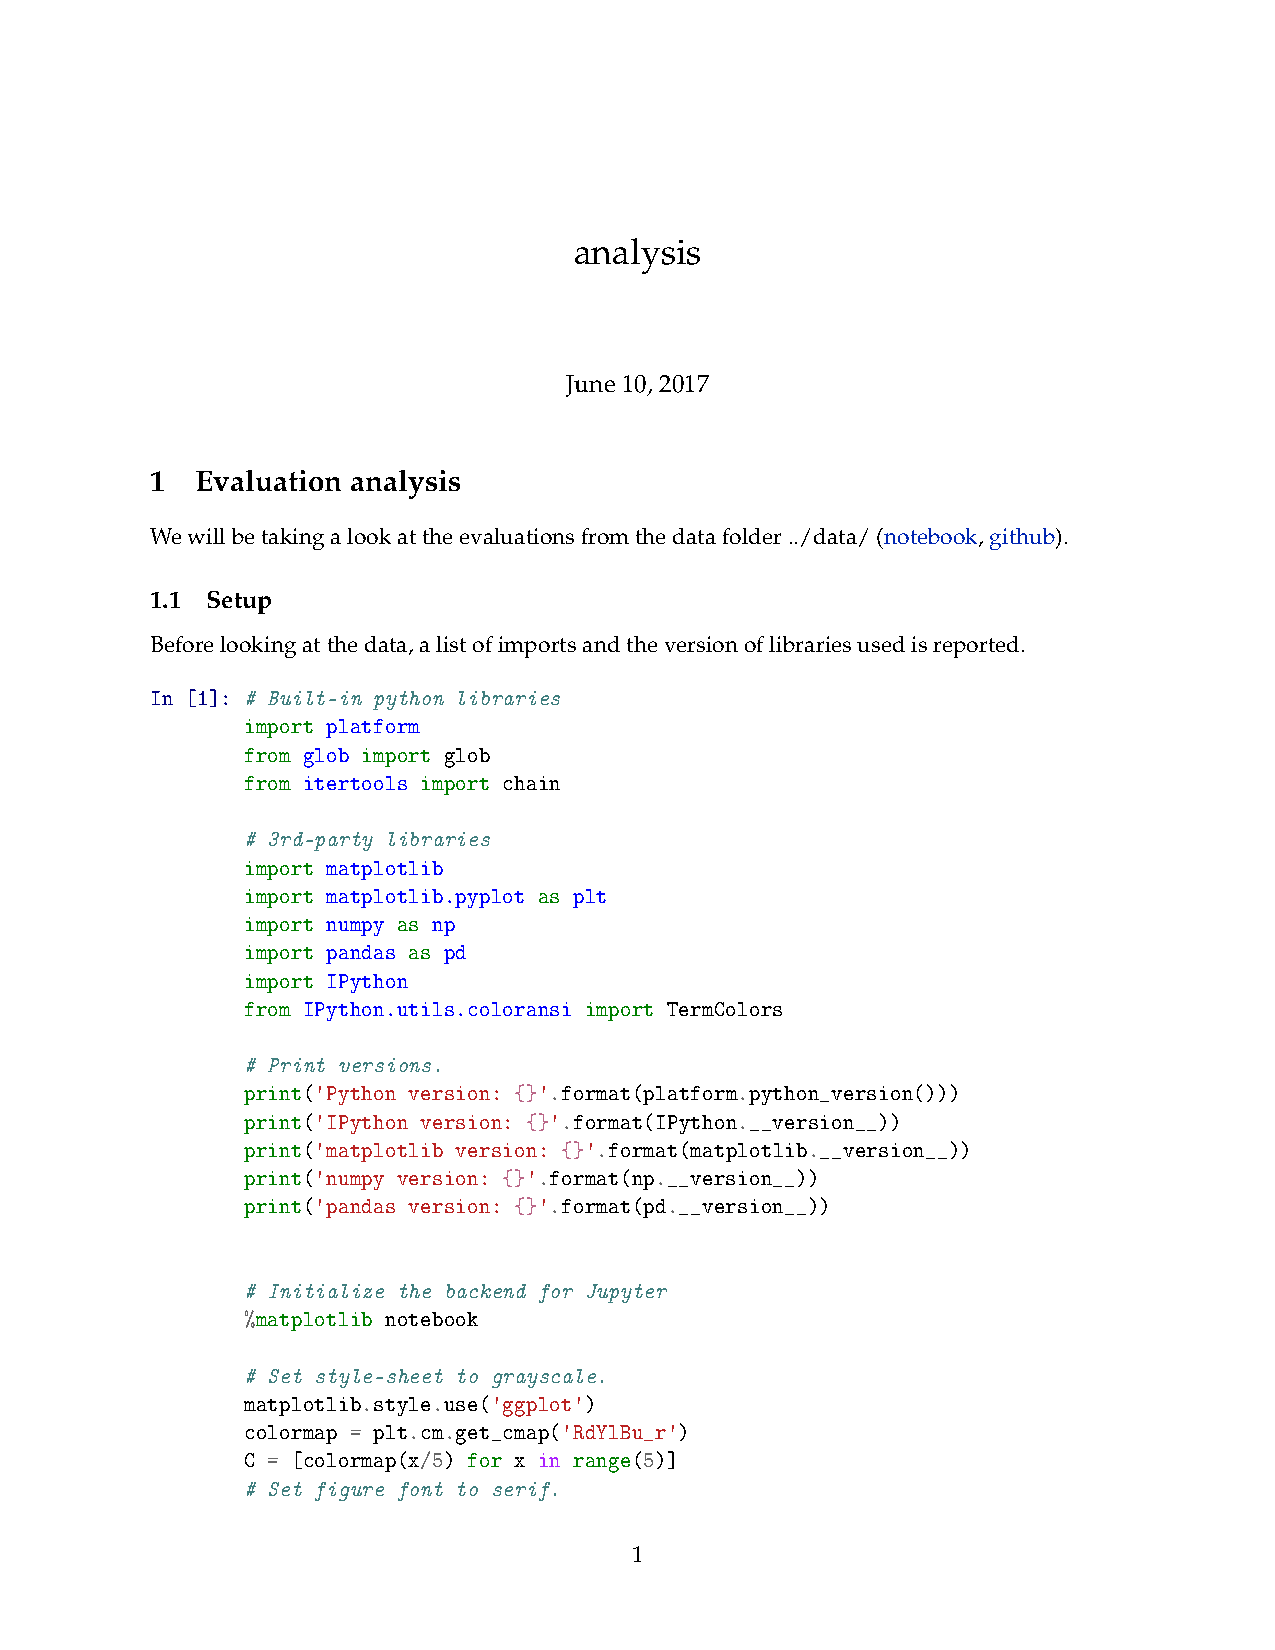
\includepdf[pages={-},scale=.8, pagecommand={}]{chapters/appendix_analysis.pdf}